\documentclass{article}
\title{Analysis report of "Design of Millimeter Wave Microstrip Reflectarrays"}
\author{Pavlo Tokariev\\Inria, I3S, Université Côte d'Azur, Sophia Antipolis}
\date{\today}


\usepackage{ulem}
\usepackage{subcaption}
\usepackage{amssymb, amsmath}
\usepackage{siunitx}
\usepackage{tikz}
\usetikzlibrary {shapes.geometric}
\usepackage{pgfplots}
\usepackage{hyperref}


\begin{document}
    \maketitle

    \begin{enumerate}
        \item First reading: introduction and conclusion (what is it about?)
        \item Second reading: the authors are brilliant! (detect good ideas)
        \begin{enumerate}
            \item the authors had a strong motivation to perform this research: which one?
            \item they established something successful in that direction that constitutes the main contribution of the article: what exactly?
            \item what makes them/you enthusiastic about this result?
        \end{enumerate}
        \item Third reading: the article has weaknesses! (scientific doubt)
        \begin{enumerate}
            \item real scope of the experimental results?
            \item justified affirmations?
            \item exaggerated extrapolations?
            \item mostly obvious results?
        \end{enumerate}
        \item Quality:
        \begin{enumerate}
            \item of course there is this "summary aspect" with the key points of
            the article, their links with the cited references, what novelty is
            offered by the article
            \item but you should also check additional information, what is
            known elsewhere about the subject, from what sources you got
            it, and what is the reliability of these sources
            \item lastly, you should have a critical view, to evaluate the real
            scope of the article, some assertions of the article may possibly
            be a little too "optimistic." Are they some extrapolations of
            external results, possibly a little abusive? is the structure of
            the article properly made with respect to the its goal? do the
            experimental results actually support the assertions? etc.
        \end{enumerate}
        \item Scientific contribution:
        \begin{enumerate}
            \item What is the scientific domain and context of the contribution
            \item In what respect is it original w.r.t. other contemporary or past
            publications?
            \item avoid recursive readings from article references to article
            references: it rapidly goes deep in the past.
            \item rather use keywords and your ability to explore bibliography
            \item Have hindsight and do not neglect to put the article into
            context
        \end{enumerate}
        \item Writing:
        \begin{enumerate}
            \item Is the introduction informative and motivating?
            \item Are experimental material and methods properly described?
            \item In the discussion, are the main affirmations actually deducible
            from their experiments and the current knowledge?
            \item Are the results actually innovative?
            \begin{enumerate}
                \item w.r.t. the year of the article,
                \item in particular w.r.t. the previous publications of the authors.
            \end{enumerate}
        \end{enumerate}
        \item Generally:
        \begin{enumerate}
            \item within 2 to 4 pages, you cannot go into all the technical details
            \item rather have hindsight in order to understand the role of each
            technical aspect within the whole contribution
            \item one (or a few) technical aspect(s) may be a major articulation
            of the contribution; in which case you should point it out and explain why this
            aspect is of major importance
            \item being concise is also part of the exercise
        \end{enumerate}
    \end{enumerate}

    General ideas or thoughts:
    \begin{enumerate}
        \item Reading 1: generally
        \item the article is about design of microstrip reflectarrays and describing shortcomings of the approach
        \item microstrip reflectarrays: microstrip is a printed patch, reflection antenna is a radio lens, antenna arrays are periodic pattern of antennas, that use wave phase shift to form beams
        \item validation: the results of reflectarray analysis are compared to the experiments (several antennas are built)
        \item the design and application are actually complex, as it requires accuracy in both solving the model and accuracy in materials and manufacturing
        \item Reading 2: positive
        \item The approach is designed to be adapted to several methods of feeding
        \item The article is of high-quality: presents the (too) technical part, approach to applied design and verification in one concise package.
        \item Features problems with different configurations: rectangular shape, for example, causes disturbance in electric field density, but collects more radiation from the feed, thus increasing spillover efficiency.
        \item Phase errors: phase shift of patches is sensitive to accuracy as the dependency between the patch size and phase is really small; non-calibrated feed and substract choice can also introduce random phase errors.
        \item Detailed description of experiments, a lot of explanations on causes of errors, but no mention of how measurements are done and their shortcomings (their accuracy and precision, number of experiment samples).
        \item The method presented can also predict radiation pattern of the antenna, which is also compared and pretty well match the experiment data.
        \item The authors admit that there are some things that they cannot explain, plus for honesty ("We are unable to explain the relatively high sidelobe levels for the reflector antenna, or the slightly low value of measured gain").
        \item Reading 3: negative
        \item There is no novelty: the authors already discussed (in a slightly more high-level manner) the idea behind the reflectarrays analysis and design in their previous papers (\cite{targonski.pozar_1994jun,pozar.metzler_1993apr}).
        \item Not mentioned: how big the reflectarray can be depending on the frequency; it seems to me, that for some frequencies and speeds of frequency modulation, wave would be a complete unsynchronized mess on output aperture.
        \item The images of reflectarrays are terrible, it is not possible to see anything (probably the images in the original publication were okay, but this is what we got in the available version).
        \item Doesn't give any numerical comparison to the state of the art, nor classical antennas.
        \item At the same time authors present the results like a justification for reflectarray feasibility, which is dishonest without direct comparison (it is possible that I am as an non-expert cannot understand the parameters, thus this point actually can be flawed).
        \item The results thought support the claims that it is possible to create a reflectarray.
        \item Scientific domain: design of antennas, analysis of reflectarrays, which are a hybrid between phased arrays and reflectors.
        \item Papers~\cite{zhuang.etal_1993jun,javor.etal_1995sep} propose another design and analysis method in 1993. They seem to discuss the same problem to me. The only difference are microstrip types. The coupling between them is compeletely discarded from the analysis in all cases, as it is considered low if there is enough distance. Thus it is not clear if the paper provide actual scientific improvement. There are actually no much development on reflectarrays, other than of these people.
        \item Writing:
        \item Introduction is great, it describes the context well, featuring high-level overview of reflectarray principle of operation, its composition, advantages (size, weight, cost, better gain with feed in comparison to just array) and disadvantages (electrical performance is poorer, design is harder, bandwidth is smaller, all in comparison to parabolic reflector; not specified how much though).
        \item Material and methods are greatly documented.
        \item Authors do not make any conclusions from the results, really. Mostly document the experiments and describe what can be done to improve it. In a way the paper is a demonstration of possibilities in a factual manner, without "selling" the approach, but thus it is hard to understand how good it really is for totally a non-expert like myself.
        \item Authors make emphasis on errors in their conclusions, and yes, they mostly make sense from the experiments: for example, same design process where conducted for different substrate materials, showing improvements after change of substrate.
        \item Or that because of steep change in phase for small change in patch size, the manufacturing is hard, and the element types should be carefully chosen.
        \item Yet there is no data supporting any problems with bandwidth, and I suppose that it is related to patches having different phase shifts for different frequencies, thus making such waves diverge from expected planar surface. Which is bad, as received not exactly the mirrored transceiver, it can be parabolic or whatever, messing up the wave as it is collected, making hard to recognize.
        \item But other than that, there are no magical claims of 100\% efficiency or something.
        \item Results do describe a design process with all the theory to compute phases, but it seems it was presented before in their respective articles, at least partially.
        \item The technical part is too technical for me, I cannot pinpoint the most important aspect.
        \item Yet, I think it is important to say that the equations described try to account for substrate characteristics and predict wave scattering, in order to lower losses.
    \end{enumerate}

    \section{Introduction}\label{sec:introduction}
    \section{Technical}\label{sec:technical}

    \begin{enumerate}
        \item Reflectarray is a substitution for parabolic antenna.
        \item Because it is flat and the output beam direction is controllable by the pattern on it, it is more flexible.
        \item Array part of the name is explained by the same working principle of beam forming as the phase arrays: by delaying the same signal in an array, the output waves from each component of such array, constructively resonate in a chosen direction, destructively resonating in others.
        \item This creates a planar beam.
        \item To see it another way: the reflectarray pattern essentially performs distance compensation for the input wave.
        \item This way changes in wave, like frequency modulation, which is used to transmit information, are observed uniformly at the aperture of the antenna.
        \item Often refers to something called "full-wave moment-method solution", but is never referenced.
        Maybe this is some foundational methods of electromagnetism, I don't know.
    \end{enumerate}
    \begin{figure}
        \centering
        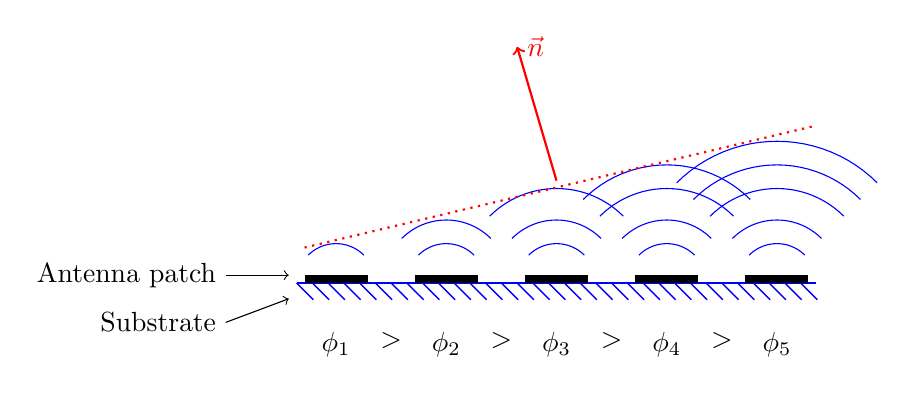
\begin{tikzpicture}
            [
            media/.style={font={\footnotesize\sffamily}},
            wave/.style={
                decorate,decoration={snake,post length=1.4mm,amplitude=2mm,
                segment length=2mm},thick},
            interface/.style={
                % The border decoration is a path replacing decorator.
                % For the interface style we want to draw the original path.
                % The postaction option is therefore used to ensure that the
                % border decoration is drawn *after* the original path.
                postaction={draw,decorate,decoration={border,angle=-45,
                amplitude=0.3cm,segment length=2mm}}},
            ]
            % Substrate
            \draw[blue,line width=.5pt,interface] (-0.1, 2) -- (6.5,2);
            % Patches
            \fill[black] (0,2) rectangle (0.8,2.1);
            \fill[black] (1.4,2) rectangle (2.2,2.1);
            \fill[black] (2.8,2) rectangle (3.6,2.1);
            \fill[black] (4.2,2) rectangle (5,2.1);
            \fill[black] (5.6,2) rectangle (6.4,2.1);

            % Waves

            \draw [blue, xshift=0.4cm, yshift=2cm, domain=45:135] plot(\x:0.5);
            \draw [blue, xshift=1.8cm, yshift=2cm, domain=45:135] plot(\x:0.5);
            \draw [blue, xshift=3.2cm, yshift=2cm, domain=45:135] plot(\x:0.5);
            \draw [blue, xshift=4.6cm, yshift=2cm, domain=45:135] plot(\x:0.5);
            \draw [blue, xshift=6.0cm, yshift=2cm, domain=45:135] plot(\x:0.5);

            %\draw [blue, xshift=0.4cm, yshift=2cm, domain=45:135] plot(\x:0.8);
            \draw [blue, xshift=1.8cm, yshift=2cm, domain=45:135] plot(\x:0.8);
            \draw [blue, xshift=3.2cm, yshift=2cm, domain=45:135] plot(\x:0.8);
            \draw [blue, xshift=4.6cm, yshift=2cm, domain=45:135] plot(\x:0.8);
            \draw [blue, xshift=6.0cm, yshift=2cm, domain=45:135] plot(\x:0.8);

            %\draw [blue, xshift=0.4cm, yshift=2cm, domain=45:135] plot(\x:1.2);
            %\draw [blue, xshift=1.8cm, yshift=2cm, domain=45:135] plot(\x:1.2);
            \draw [blue, xshift=3.2cm, yshift=2cm, domain=45:135] plot(\x:1.2);
            \draw [blue, xshift=4.6cm, yshift=2cm, domain=45:135] plot(\x:1.2);
            \draw [blue, xshift=6.0cm, yshift=2cm, domain=45:135] plot(\x:1.2);

            %\draw [blue, xshift=0.4cm, yshift=2cm, domain=45:135] plot(\x:1.5);
            %\draw [blue, xshift=1.8cm, yshift=2cm, domain=45:135] plot(\x:1.5);
            %\draw [blue, xshift=3.2cm, yshift=2cm, domain=45:135] plot(\x:1.5);
            \draw [blue, xshift=4.6cm, yshift=2cm, domain=45:135] plot(\x:1.5);
            \draw [blue, xshift=6.0cm, yshift=2cm, domain=45:135] plot(\x:1.5);

            %\draw [blue, xshift=0.4cm, yshift=2cm, domain=45:135] plot(\x:1.8);
            %\draw [blue, xshift=1.8cm, yshift=2cm, domain=45:135] plot(\x:1.8);
            %\draw [blue, xshift=3.2cm, yshift=2cm, domain=45:135] plot(\x:1.8);
            %\draw [blue, xshift=4.6cm, yshift=2cm, domain=45:135] plot(\x:1.8);
            \draw [blue, xshift=6.0cm, yshift=2cm, domain=45:135] plot(\x:1.8);

            \draw [red, thick, dotted] (0, 2.45) -- (6.5, 4);
            \draw [red, thick, ->] (3.2, 3.3) -- (2.7,5) node[right] {$\vec{n}$};
            % Legend
            \draw[black, ->] (-1,1.5) node[left] {Substrate} -- (-0.2,1.8);
            \draw[black, ->] (-1,2.1) node[left] {Antenna patch} -- (-0.2,2.1);

            \filldraw[black] (0.4,1.5) circle (0pt) node[below]{$\phi_1$};
            \filldraw[black] (1.1,1.5) circle (0pt) node[below]{$>$};
            \filldraw[black] (1.8,1.5) circle (0pt) node[below]{$\phi_2$};
            \filldraw[black] (2.5,1.5) circle (0pt) node[below]{$>$};
            \filldraw[black] (3.2,1.5) circle (0pt) node[below]{$\phi_3$};
            \filldraw[black] (3.9,1.5) circle (0pt) node[below]{$>$};
            \filldraw[black] (4.6,1.5) circle (0pt) node[below]{$\phi_4$};
            \filldraw[black] (5.3,1.5) circle (0pt) node[below]{$>$};
            \filldraw[black] (6.0,1.5) circle (0pt) node[below]{$\phi_5$};
        \end{tikzpicture}
        \caption{Phase array}
        \label{fig:phase_array}
    \end{figure}
    \begin{figure}
        \centering
        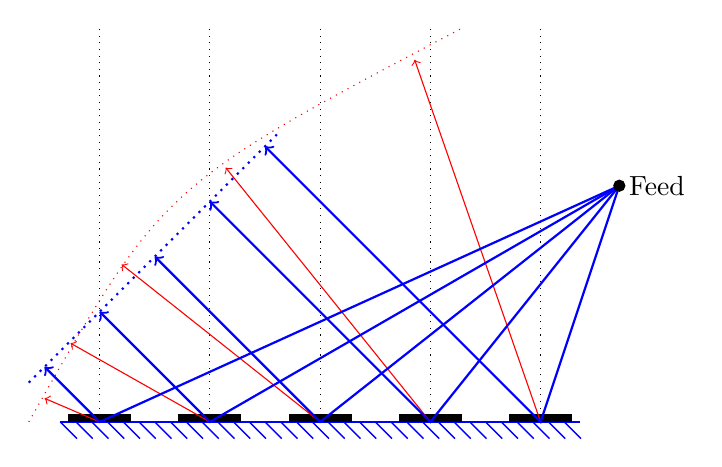
\begin{tikzpicture}
            [
            media/.style={font={\footnotesize\sffamily}},
            wave/.style={
                decorate,decoration={snake,post length=1.4mm,amplitude=2mm,
                segment length=2mm},thick},
            interface/.style={
                % The border decoration is a path replacing decorator.
                % For the interface style we want to draw the original path.
                % The postaction option is therefore used to ensure that the
                % border decoration is drawn *after* the original path.
                postaction={draw,decorate,decoration={border,angle=-45,
                amplitude=0.3cm,segment length=2mm}}},
            ]
            % Substrate
            \draw[blue,line width=.5pt,interface] (-0.1, 2) -- (6.5,2);

            % Axis
            \draw[black,dotted] (0.4,2) -- (0.4,7);
            \draw[black,dotted] (1.8,2) -- (1.8,7);
            \draw[black,dotted] (3.2,2) -- (3.2,7);
            \draw[black,dotted] (4.6,2) -- (4.6,7);
            \draw[black,dotted] (6.0,2) -- (6.0,7);

            % Patches
            \fill[black] (0,2) rectangle (0.8,2.1);
            \fill[black] (1.4,2) rectangle (2.2,2.1);
            \fill[black] (2.8,2) rectangle (3.6,2.1);
            \fill[black] (4.2,2) rectangle (5,2.1);
            \fill[black] (5.6,2) rectangle (6.4,2.1);



            % Reflected wave
            \draw[red,->] (0.4,2) -- (-0.3,2.3);
            \draw[red,->] (1.8,2) -- (0.03,3);
            \draw[red,->] (3.2,2) -- (0.68,4);
            \draw[red,->] (4.6,2) -- (2,5.23);
            \draw[red,->] (6.0,2) -- (4.4,6.6);
            \draw[red,dotted] (-0.5,2) .. controls (1.2,5) .. (5,7);

            % Expected wave
            \draw[blue,thick,dotted] (-0.5,2.5) -- (2.7,5.7);
            \draw[blue,thick,->] (7,5) -- (0.4,2) -- (-0.3,2.7);
            \draw[blue,thick,->] (7,5) -- (1.8,2) -- (0.4,3.4);
            \draw[blue,thick,->] (7,5) -- (3.2,2) -- (1.1,4.1);
            \draw[blue,thick,->] (7,5) -- (4.6,2) -- (1.8,4.8);
            \draw[blue,thick,->] (7,5) -- (6.0,2) -- (2.5,5.5);

            % Feed
            \filldraw[black] (7,5) circle (2pt) node[right]{Feed};

        \end{tikzpicture}
        \caption{Reflectarray}
        \label{fig:reflectarray}
    \end{figure}
    \section{Conclusion}\label{sec:conclusion}

    \section{Quality}\label{sec:quality}

    \subsection{References}\label{subsec:references}
    \begin{enumerate}
        \item self-citation: 6/15 references, seems to be not bad.
        \item reflect array concept\cite{berry.etal_1963nov}.
        This citation is actually the original publication featuring reflectarrays.
        \item claim: "losses in a microstrip feed network in a large array at high frequencies are often unacceptable" citation 2 is unavailable in free access, so cannot check.
        The claim makes sense in all antennas by the way, losses are unacceptable.
        \item "stubs of variable length to control the reflection phase"~\cite{munson.etal_1987aug,huang_1991jun,chang.huang_1992}.
        This is true, the papers do present what is claimed, yet the lastest is unavailable in free access.
        \item "A better approach, and the one used for the present work, is to use printed dipoles or patches of variable size to control the phase"~\cite{pozar.metzler_1993apr,targonski.pozar_1994jun}.
        First is not freely available.
        \sout{I am not convinced what is that good about the new method.}
        Bandwidth of the patched is not as restricted as for patches with stubs, the grid doesn't have to be triangular.
        \item Feeling that the authors write the same things over and over again in their papers.
        \item "The procedure is very similar to the analysis of radar cross section of a microstrip antenna to~\cite{pozar_1987jun} and the analysis of infinite arrays of microstrip elements"~\cite{harackiewicz_1990jan}, one reference is not available at all, not possible to find.
        The claim matches the references' abstracts (body of the thesis is not available).
        \item "Using the definitions in~\cite{balanis_1982}",  cannot check, unavailable.
        \item "transformation from a plane wave field to a spherical wave, and is related to the radar cross section of a square plate~\cite{knott.etal_2004}" --- unvailable.
        \item "surface wave loss for a single microstrip element on a low-dielectric constant substrate is typically less than 15\%"\cite{pozar_1985oct} --- don't see the claim in the reference.
        From the fast reading of the results, it seems that losses can very greatly, from almost none, to 70\%.
        \item "Some estimates suggest that the variation of loss tangent is approximately linear with frequency\cite{levine.etal_1989apr}" --- cannot find the claim, the conclusion and the data presented do not mention frequency modulation at all.
        \item "circular waveguide-fed dielectric cap~\cite{syrigos_1987jun}" -- yeah, matches.
    \end{enumerate}
    \bibliographystyle{plain}
    \bibliography{refs}
\end{document}
